\section{Szczegóły implementacyjne}
\label{sec:szczegoly-implementacyjne}
Projekt jest realizowany na platformie FPGA. Układy FPGA, w przeciwieństwie do procesorów CPU, nie mają z góry ustalonej struktury -- schemat układu jest programowalny. Daje to możliwość projektowania wysoce wyspecjalizowanych układów, które będą miały strukturę zoptymalizowaną pod kątem wykonywania konkretnego zadania. Takie podejście jest znacząco różne od procesorów CPU, które są w stanie wykonywać jedynie z góry określone zestawy instrukcji ogólnego przeznaczenia. Programy wykonywane na CPU są ciągiem takich operacji.

\subsection{Wykorzystane technologie oraz narzędzia programistyczne}
Projekt jest realizowany na platformie FPGA, więc musi zostać napisany w języku opisu sprzętu. Wykorzystany został język VHDL, ze względu na jego silną kontrolę typów, która pozwala na wczesne wykrywanie niektórych błędów podczas kompilacji, co okazało się bardzo pomocne podczas implementowania modułów AES.

Środowiskiem programistycznym, które zostało wykorzystane do realizacji tego projektu jest Altera Quartus Prime 15.1 Lite Edition. Taki wybór był podyktowany faktem, że wykorzystana w projekcie płytka Terasic DE1-SOC wyposażona jest w układ FPGA firmy Altera, a Quartus jest jedynym środowiskiem przeznaczonym do tworzenia oprogramowania dla układów FPGA tej firmy.

Do realizacji projektu zostało wykorzystane narzędzie QSys, które wchodzi w skład środowiska Quartus oraz służy do integracji zasobów dostępnych na płytce w projekcie, np. HPS, RAM. Pozwala również na konfigurację tych komponentów, co ma kluczowe znaczenie dla wykorzystania znajdującego się na płytce konwertera USB UART (rozdz. \ref{sec:uart-qsys}).

Do przygotowania karty SD wykorzystane zostało środowisko Altera SoC FPGA Embedded Design Suite 15.1, które zawiera narzędzia programistyczne przeznaczone do tworzenia projektów korzystających zarówno z programowalnej części FPGA jak i procesora HPS. Użyte zostało narzędzie \textit{bsp-editor}, które posłużyło do wygenerowania preloadera (rozdz. \ref{sec:uart-preloader-gen}).

Testy implementowanych komponentów były realizowane jako symulacje funkcyjne przy pomocy narzędzi wchodzących w skład środowiska programistycznego Quartus.


\subsection{Przygotowanie oraz konfiguracja projektu}
\label{sec:przygotowanie-projektu}

Terasic -- producent wykorzystanej w tym projekcie płytki płytki DE1-SOC -- opracował i udostępnił na płycie CD dołączonej do zestawu \cite{terasic-cd} projekt bazowy GHRD (ang. \textit{Golden Hardware Reference Design}). Jest to projekt skonfigurowany do poprawnego działania z płytką DE1-SOC, w którym ustawione są m.in.
\begin{itemize}[noitemsep]
\item model układu FPGA znajdującego się na płytce
\item konfiguracja pinów
\item podstawowe ograniczenia czasowe układu
\item projekt QSys reprezentujący zintegrowany procesor HPS (ang. \textit{Hard Processor System})
\item główny plik projektu (ang. \textit{top-level entity}) wraz z dodanym komponentem reprezentującym HPS
\end{itemize}
Projekt GHRG zawiera podstawowe ustawienia, więc umożliwia programiście skrócenie etapu konfiguracji projektu oraz szybkie rozpoczęcie pracy nad projektowanym układem. Bazą dla tego projektu był GHRD.

Do konwersji sygnału USB do UART wykorzystany został znajdujący się na płytce Terasic DE1-SOC układ firmy FTDI. Jego sygnały nie są jednak podłączone bezpośrednio do programowalnej części układu FPGA, lecz do zintegrowanego procesora ARM. Aby uzyskać dostęp do jego sygnałów z FPGA należy odpowiednio dostosować projekt (rozdz. \ref{sec:uart-qsys}) oraz stworzyć i wgrać na kartę SD preloader (rozdz. \ref{sec:uart-preloader-gen}), który podczas uruchamiania płytki przestawi piny UART w odpowiedni tryb działania oraz określi ich kierunek.

\subsubsection{Konfiguracja pinów UART}
\label{sec:uart-qsys}
Aby skonfigurować projekt tak, aby układ FPGA miał dostęp do sygnałów UART konwertera USB UART podłączonych do HPS, należy wykonać następujące czynności \cite{altera-youtube-loanerio, altera-forum-fgga-hps-access, altera-forum-cant-rx}:

\begin{enumerate}
\item Otworzyć w edytorze QSys plik \textit{soc-system.qsys}
\item Wybrać komponent \textit{hps\_0} (rys. \ref{fig:qsys-hps} A) oraz w zakładce \textit{Peripheral Pins} (rys. \ref{fig:qsys-hps} B) dokonać zmian:
	\begin{itemize}[noitemsep,nolistsep]
	\item Zmienić wartość \textit{UART0 pin} na \textit{FPGA} (rys. \ref{fig:qsys-hps} C)
	\item Zmienić wartość \textit{UART0 mode} na \textit{Full} (rys. \ref{fig:qsys-hps} C)
	\item Zaznaczyć \textit{LOANIO 49} oraz \textit{LOANIO 50} (rys. \ref{fig:qsys-hps} D)
	\end{itemize}
\item Opcjonalnie można oczyścić projekt z komponentów, które zostały skonfigurowane w GHRD a nie zostaną wykorzystane: \textit{dipsw\_pio}, \textit{button\_pio}, \textit{led\_pio}.
\item Zapisać zmiany, wygenerować kod VHDL klikając przycisk \textit{Generate HDL...} (rys. \ref{fig:qsys-hps} E) oraz opuścić edytor (rys. \ref{fig:qsys-hps} F).
\item W głównym pliku projektu (ang. \textit{Top-Level Entity}) zmodyfikować komponent \textit{soc-system} tak, aby był zgodny z jego na nowo wygenerowaną wersją.
\item Przypisać wartość \textit{'1'} sygnałom:
	\begin{itemize}[noitemsep,nolistsep]
	\item \textit{hps\_0\_uart0\_cts}
	\item \textit{hps\_0\_uart0\_dsr}
	\item \textit{hps\_0\_uart0\_dcd}
	\item \textit{hps\_0\_uart0\_ri}
	\item \textit{hps\_0\_uart0\_rxd}
	\end{itemize}
\item Sygnał \textit{hps\_0\_hps\_io\_hps\_io\_gpio\_inst\_LOANIO49} przypisać do pinu \textit{HPS\_UART\_RX}.
\item Sygnał \textit{hps\_0\_hps\_io\_hps\_io\_gpio\_inst\_LOANIO50} przypisać do pinu \textit{HPS\_UART\_TX}.
\item Wektor sygnałów \textit{hps\_0\_h2f\_loan\_io\_oe} określa kierunek pinów pinów \textit{LOANIO}.
	\begin{itemize}[noitemsep,nolistsep]
	\item Do sygnału \textit{hps\_0\_h2f\_loan\_io\_oe(49)}, który odpowiada sygnałowi UART RX przypisać wartość \textit{'1'}, co odpowiada kierunkowi \textit{out}.
	\item Do sygnału \textit{hps\_0\_h2f\_loan\_io\_oe(50)}, który odpowiada sygnałowi UART TX przypisać wartość \textit{'0'}, co odpowiada kierunkowi \textit{in}.
	\end{itemize}
\end{enumerate}

\begin{figure}[!h]
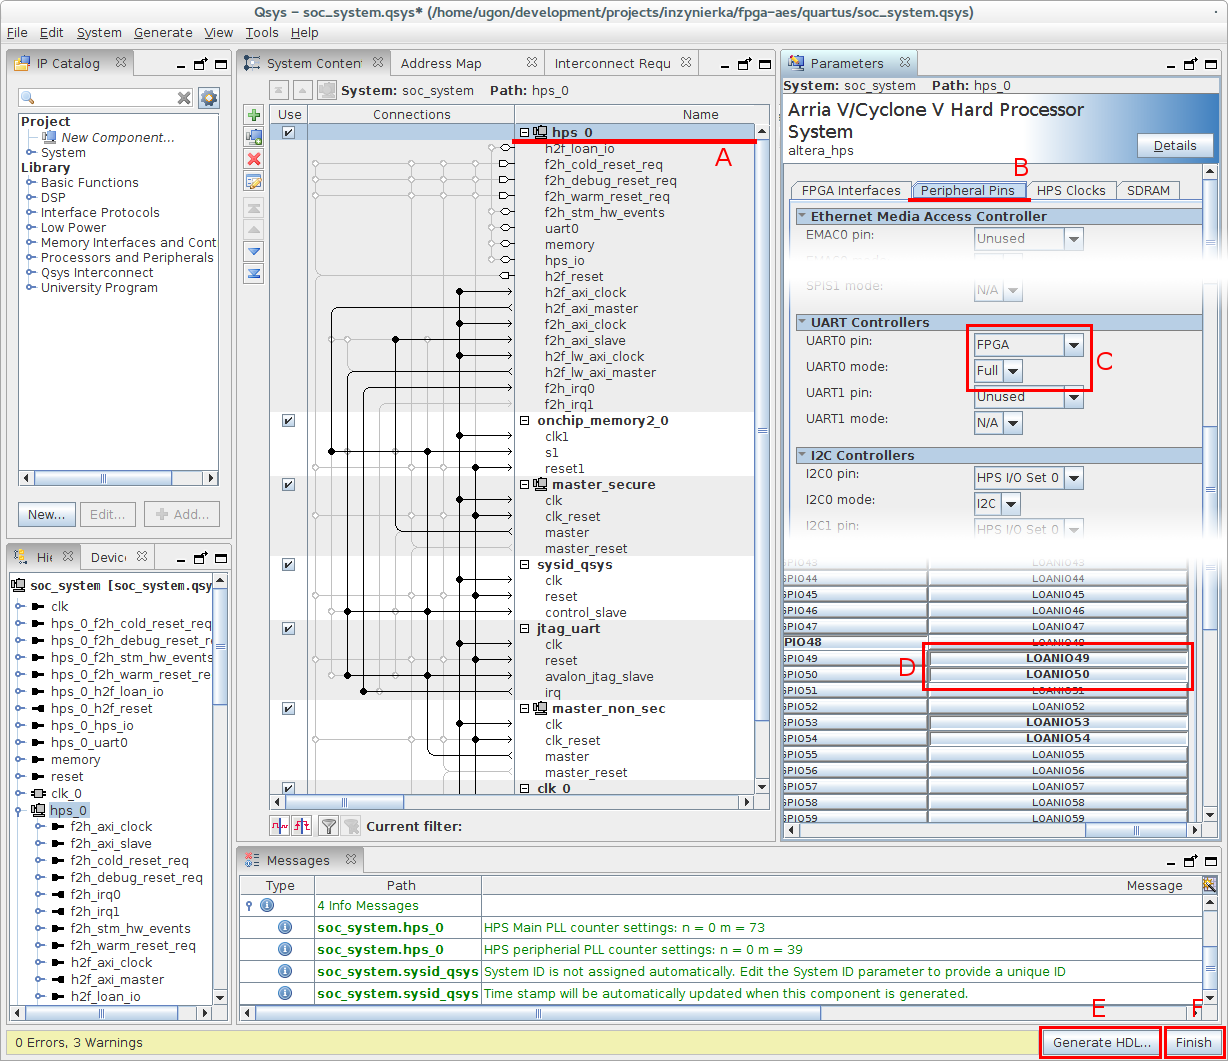
\includegraphics[width=\textwidth]{pictures/qsys.png}
\caption{Konfiguracja komponentu HPS w edytorze QSys}
\label{fig:qsys-hps}
\end{figure}

Wykonane zmiany spowodują, że:
\begin{itemize}[noitemsep]
\item Sygnał \textit{hps\_0\_h2f\_loan\_io\_out(49)} będzie odpowiadał sygnałowi UART RX oraz będzie poprawnie połączony z konwerterem USB-UART firmy FTDI.
\item Sygnał \textit{hps\_0\_h2f\_loan\_io\_out(50)} będzie odpowiadał sygnałowi UART TX oraz będzie poprawnie połączony z konwerterem USB-UART firmy FTDI
\end{itemize}


\subsubsection{Przygotowanie preloadera}
\label{sec:uart-preloader-gen}
Aby przy starcie płytki piny UART zostały poprawnie połączone z układem FPGA należy z plików powstałych w wyniku kompilacji projektu wygenerować preloader. Aby to zrobić można posłużyć się narzędziem \textit{bsp-editor} będącym częścią oprogramowania Quartus, zgodnie z instrukcją znalezioną w internecie \cite{rocketboards-preloader}.

\subsubsection{Skrypt startowy programujący układ FPGA}
Aby automatycznie zaprogramować układ FPGA podczas startu urządzenia używany jest skrypt, który będzie się wykonywał w fazie startowej U-Boot \cite{rocketboards-uboot-script}.
\begin{lstlisting}
fatload mmc 0:1 $fpgadata soc_system.rbf;
fpga load 0 $fpgadata $filesize;
\end{lstlisting}

\begin{figure}[!h]
\centering
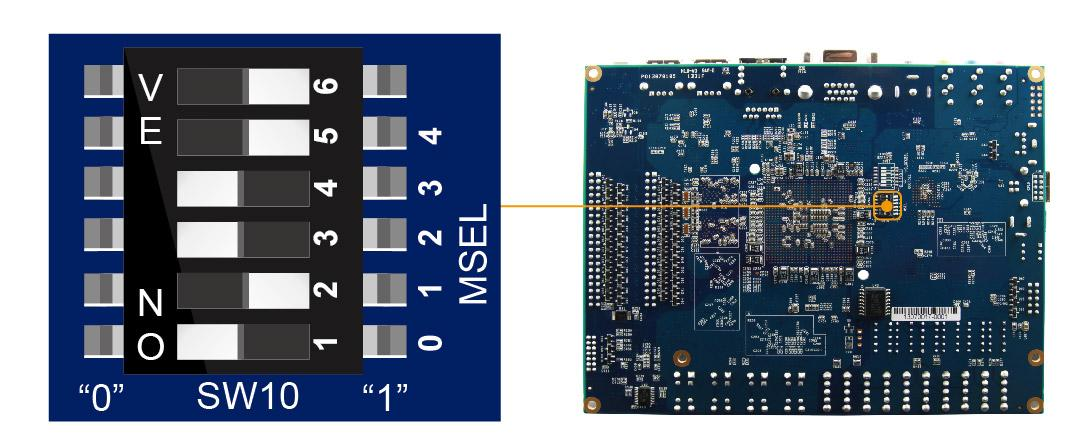
\includegraphics[width=\textwidth]{pictures/msel.png}
\caption{Przełączniki MSEL[0:4] na płytce Terasic DE1-SOC}
\label{fig:msel}
\end{figure}

Do programowania układu FPGA przy pomocy skryptu potrzebny jest plik konfiguracyjny w formacie \textit{.rbf}. Można go stworzyć konwertując przy pomocy środowiska Quartus plik \textit{.sof} powstały w wyniku kompilacji projektu \cite{rocketboards-sof-to-rfb}. W tym projekcie używany jest tryb programowania \textit{Fast Passive Parallel X16}, któremu odpowiada ustawienie przełączników MSEL[0:4] znajdujących się na płytce (rys. \ref{fig:msel}) na wartość 00100.

\subsubsection{Przygotowanie karty SD}
Najłatwiejszym sposobem na stworzenie karty SD zawierającej potrzebne pliki jest modyfikacja dostarczonych na płycie CD do płytki Terasic DE1-SOC przykładowych obrazów. Lista kroków realizujących to zadanie przy użyciu komputera z systemem operacyjnym Linux \cite{rocketboards-booting-prebuild, rocketboards-updating-sd}:
\begin{enumerate}
\item Po włożeniu karty SD do czytnika należy określić jej ścieżkę w systemie operacyjnym, najlepiej analizując plik \textit{/proc/partitions}. Załóżmy, że ścieżką karty jest \textit{/dev/sdx}.
\begin{lstlisting}
  $ cat /proc/partitions
\end{lstlisting}

\item Wgrać dostarczony przez producenta obraz \textit{DE1\_SoC\_SD.img} \cite{terasic-sd} na kartę SD.
\begin{lstlisting}
  $ sudo dd if=DE1\_SoC\_SD.img of=/dev/sdx bs=1M
  $ sudo sync
\end{lstlisting}

\item Zastąpić domyślny preloader
\begin{lstlisting}
  $ sudo dd if=preloader-mkpimage.bin of=/dev/sde3 bs=64k seek=0
  $ sudo sync
\end{lstlisting}

\item Wgrać skrypt U-Boot oraz plik zawierający konfigurację układu FPGA na partycję FAT \textit{/dev/sdx1} dowolnym sposobem (np. korzystając z systemowego eksploratora plików).
\end{enumerate}

Aby przy starcie płytki programowanie FPGA przebiegło pomyślnie, należy umieścić kartę SD w czytniku oraz ustawić przełączniki MSEL[4:0] (rys. \ref{fig:msel}) w pozycji 00100.

\subsubsection{Ograniczenia czasowe}
Aby mieć gwarancję, że projekt nie będzie zachowywał się niedeterministyczne ze względu na złe ułożenie ścieżek sygnałów w chipie FPGA powodujące zbyt długi czas propagacji, zdefiniowane zostały odpowiednie ograniczenia czasowe. Do tego celu posłużyła konsola w narzędziu TimeQuest Timing Analyzer będącym częścią środowiska programistycznego Quartus. Zdefiniowane ograniczenia to:

\begin{itemize}
\item Zewnętrzny zegar \textit{CLK\_50} o częstotliwości 50MHz
\begin{lstlisting}[basicstyle=\footnotesize]
create_clock -name {CLK_50} -period 20.000 { CLOCK_50 }
\end{lstlisting}

\item Główny zegar projektu \textit{CLK\_16} (rozdz. \ref{sec:clk-16})
\begin{lstlisting}[basicstyle=\footnotesize]
create_generated_clock -name {CLK_16} -source {CLOCK_50} 
	-divide_by 26 { uart_prescaler0|clk|q }
\end{lstlisting}

\item Sygnał w module \textit{block\_serializer} (rozdz. \ref{sec:block-serializer}), na którego zbocze rosnące musiał być wrażliwy proces sterujący sygnałem zakończenia wysyłania bloku -- \outsignal{FINISHED\_TRANSMITTING}.
\begin{lstlisting}[basicstyle=\footnotesize]
create_generated_clock -name {SERIALIZER_CLK} 
	-source {uart_prescaler0|clk|q} -divide_by 2 -offset 260.000 
	{ communicator0|block_serializer0|forward_start|q }
\end{lstlisting}

\item Sygnał w module \textit{block\_deserializer} (rozdz. \ref{sec:block-deserializer}), na którego zbocze rosnące musiał być wrażliwy proces sterujący sygnałami odebranego bloku \outsignal{AES\_BLOCK[127:0]} oraz zakończenia odbierania \outsignal{FINISHED\_LISTENING}.
\begin{lstlisting}[basicstyle=\footnotesize]
create_generated_clock -name {DESERIALIZER_CLK} \
	-source {uart_prescaler0|clk|q} -divide_by 2 -offset 260.000 
	{ communicator0|block_deserializer0|forward_finished|q }
\end{lstlisting}

\end{itemize}

Są to wszystkie sygnały pełniące w tym projekcie rolę zegarów.

\subsection{Główny zegar}
\label{sec:clk-16}
Główny zegar \textit{CLK\_16}, którym taktowany będzie projektowany układ ma częstotliwość
\begin{equation}
f_{CLK\_16} = 16 * UART\_BAUD\_RATE
\end{equation}
gdzie \textit{UART\_BAUD\_RATE} jest szybkością transmisji sygnału UART wyrażoną w baudach, która dla tego projektu wynosi 115200 baudów. Taka wartość podyktowana jest faktem, że częstą praktyką interpretacji sygnału UART, jest jego próbkowanie z częstotliwością 16 razy szybszą niż częstotliwość zmian sygnału.

Częstotliwość zegara \textit{CLK\_16} jest o wiele niższa niż dostępny w układzie FPGA zegar o częstotliwości 50MHz. Pozwoliło to na uzyskanie żądanej częstotliwości przy pomocy prostego dzielnika częstotliwości (listing 1).

\begin{figure}[!h]
\begin{lstlisting}[style=vhdl, caption={Dzielnik częstotliwości \textit{uart\_prescaler}}, captionpos=b]
entity uart_prescaler is
	port (
		clk_in  : in  std_logic;  --50MHz
		clk_out : out std_logic); --16 * 115200Hz
end uart_prescaler;

architecture uart_prescaler_impl of uart_prescaler is
	signal clk : std_logic := '0';
begin
	clk_out <= clk;
	
	process (clk_in) 
		variable counter : Integer range 0 to 13 := 0;
	begin	
		if(rising_edge(clk_in)) then
			case counter is
				when 13 =>
					clk <= not clk;
					counter := 0;
				when others =>
					counter := counter + 1;
			end case;
		end if;
	end process;
end uart_prescaler_impl;
\end{lstlisting}
\end{figure}

Układ jest wyzwalany rosnącymi zboczami zegara \textit{CLK\_16}. Jeśli akcja mająca miejsce w danym rosnącym zboczu zależy od wartości innego sygnału, to ma on stałą wartość co najmniej od poprzedzającego do następnego zbocza malejącego.

\subsection{Synchronizacja sygnału UART RX}
\label{uart-sync}
Sygnał UART RX pochodzi z peryferyjnego konwertera USB-UART firmy FTDI, który jest w domenie innego zegara. Powoduje to, że w momencie wystąpienia zbocz rosnących lub malejących głównego zegara, sygnał RX może nie mieć dobrze określonej wartości (np. również być w trakcie zbocza). Może to prowadzić do wystąpienia stanów metastabilnych \cite{altera-metastability} i w efekcie doprowadzić do niedeterministycznego działania układu. Aby temu zapobiec sygnał RX został zsynchronizowany przy pomocy dwóch przerzutników typu D wyzwalanych głównym zegarem \cite{altera-metastability, 2ff-synchronization} (rys. \ref{fig:2ff}). Jest to standardowa technika, która powoduje drastyczne zmniejszenie prawdopodobieństwa wystąpienia stanów metastabilnych z powodu używania sygnałów pochodzących z domen innych zegarów.

\begin{figure}[!h]
\centering
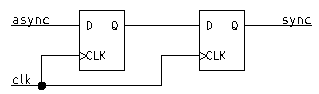
\includegraphics[width=100mm,scale=1.5]{pictures/2ff.pdf}
\caption{Synchronizacja sygnału przy użyciu dwóch przerzutników typu D}
\label{fig:2ff}
\end{figure}

\begin{figure}[!h]
\centering
\begin{tikztimingtable}
  \textit{CLK\_16}   & cc 16{cc}     16{cc}       7{c}       \\
  \textit{RX}        & hh 16J{Start} 16D{DATA[0]} 7d{Data[1]}\\
\extracode
\tablerules
\vertlines[red]{1}
\vertlines[red]{17}
\vertlines[red]{33}
\end{tikztimingtable}
\caption{Relacja między zegarem \textit{CLK\_16} i zsynchronizowanym sygnałem \textit{RX}}
\label{fig:clk-rx-sync}
\end{figure}

Przerzutniki są wyzwalane zboczami malejącymi zegara \textit{CLK\_16}. Powoduje to, że sygnał \textit{RX} zmienia wartość podczas zbocz malejących oraz jest stabilny podczas zbocz rosnących tego zegara (rys. \ref{fig:clk-rx-sync}). Takie zachowanie sygnału jest wymagane przez moduł \textit{uart\_rx} (rozdz. \ref{sec:uart-rx}).


